\documentclass{article}
\title{ECE 478-- Homework 5}
\usepackage{graphicx}
\usepackage{fancyhdr}
\usepackage{enumitem}
\usepackage{amsmath}
\usepackage{amssymb}
\usepackage{float}
\usepackage{amsmath}
\usepackage[margin=1in]{geometry}
\pagestyle{fancy}
\fancyhf{}
\fancyhead[L]{Gianni Avilan-Losee}
\fancyhead[C]{ECE 478}
\fancyhead[R]{Homework 5}
\fancyfoot[C]{\thepage}
\usepackage{microtype}
\usepackage{textcomp, gensymb}
\author{Gianni Avilan-Losee}
\begin{document}
\setcounter{section}{6}
\setcounter{subsection}{1}
\begin{enumerate}[label=\thesubsection]
	\item Simplifying the wire under consideration to a uniform slab of material, we may use \textit{sheet resistance} to easily derive the resistance of the material per unit length.

		First, to find the sheet resistance, we will need the material's resistivity as well as its thickness, while incorporating the thickness of the barrier material. Using Table 6.2, we may estimate the bulk resistivity of Cu at \(22\degree \ \mathrm{C}\) as \(1.7 \ \micro\ohm \cdot \mathrm{cm}\). Assuming that barrier material is included in the parameters given by Table 6.1, this reduces the effective thickness of the M1 layer in the Intel 45 nm stack to \(144 - 10 = 134 \ \mathrm{nm}\). Then, calculating the sheet resistance,
		\[
			R_{\square} = \frac{\rho}{t-t_{\mathrm{barrier}}} = \frac{1.7 \micro\ohm \cdot \mathrm{cm}}{134 \ \mathrm{nm}} = 1.27 \times 10^5 \ \frac{\micro\ohm}{\square} = 127 \ \frac{\mathrm{m}\ohm}{\square}.
		\]
		This refers to the resistance of a slab of equal length and width for the given material, regardless of dimensions used. 

		Then, multiplying sheet resistance by a length of \(1 \ \mathrm{mm}\) and dividing by width, once again reducing the effective width by \(2t_{\mathrm{barrier}}\), since the conductive material is surrounded on either side by a \(10 \ \mathrm{nm}\) layer of barrier material, 
		\[
			R_{\mathrm{per \ mm}} = R_{\square}\frac{l}{w - 2t_{\mathrm{barrier}}} = (127 \ \frac{\mathrm{m}\ohm}{\square}) \ \frac{1 \ \mathrm{mm}}{60 \ \mathrm{nm}} = 2.117 \times 10^3 \ \ohm.
		\]
		Recalculating for each relevant pitch (as some are repeated), 
		\begin{align*}
			&\mathrm{pitch \ (nm)} &R_{\mathrm{per \ mm}} \ (\ohm) \\
			&240 &820 \\
			&280 &585 \\
			&360 &338 \\
			&560 &132 \\
			&720 &63 \\
			&7 \times 10^3 &0.139 \\
		\end{align*}
	\setcounter{subsection}{2}
\item For the wire in the \(pi\)-model, we can use the sheet resistance to derive total resistance, and the given capacitance per unit length to derive the capacitance on each side of the wire's resistance. Finding the resistance first, we'll use \(\lambda = 0.3 \ \micro\mathrm{m}\) to find width \(w = 0.3 \times 4 = 1.2 \ \micro\mathrm{m} = 1.2 \times 10^{-3} \ \mathrm{mm}\). Then,
		\[
			R_{\mathrm{wire}} = R_{\square} \ \frac{l}{w} = 0.08 \times \frac{5}{1.2 \times 10^{-3}} = 333.34 \ \ohm.
		\]
		Then, using capacitance per unit length of \(C = 0.2 \ \mathrm{\frac{fF}{\micro m}}\), 
		\[
			C_{\mathrm{wire}} = (0.2 \times 10^{-15})(5 \times 10^{3}) = 1 \times 10^{-12} = 1 \ \mathrm{pF}.
		\]
		Fig. 1 shows the corresponding \(\pi\)-model representation of the wire with the above parameters.
\begin{figure}[H]
  \centering
  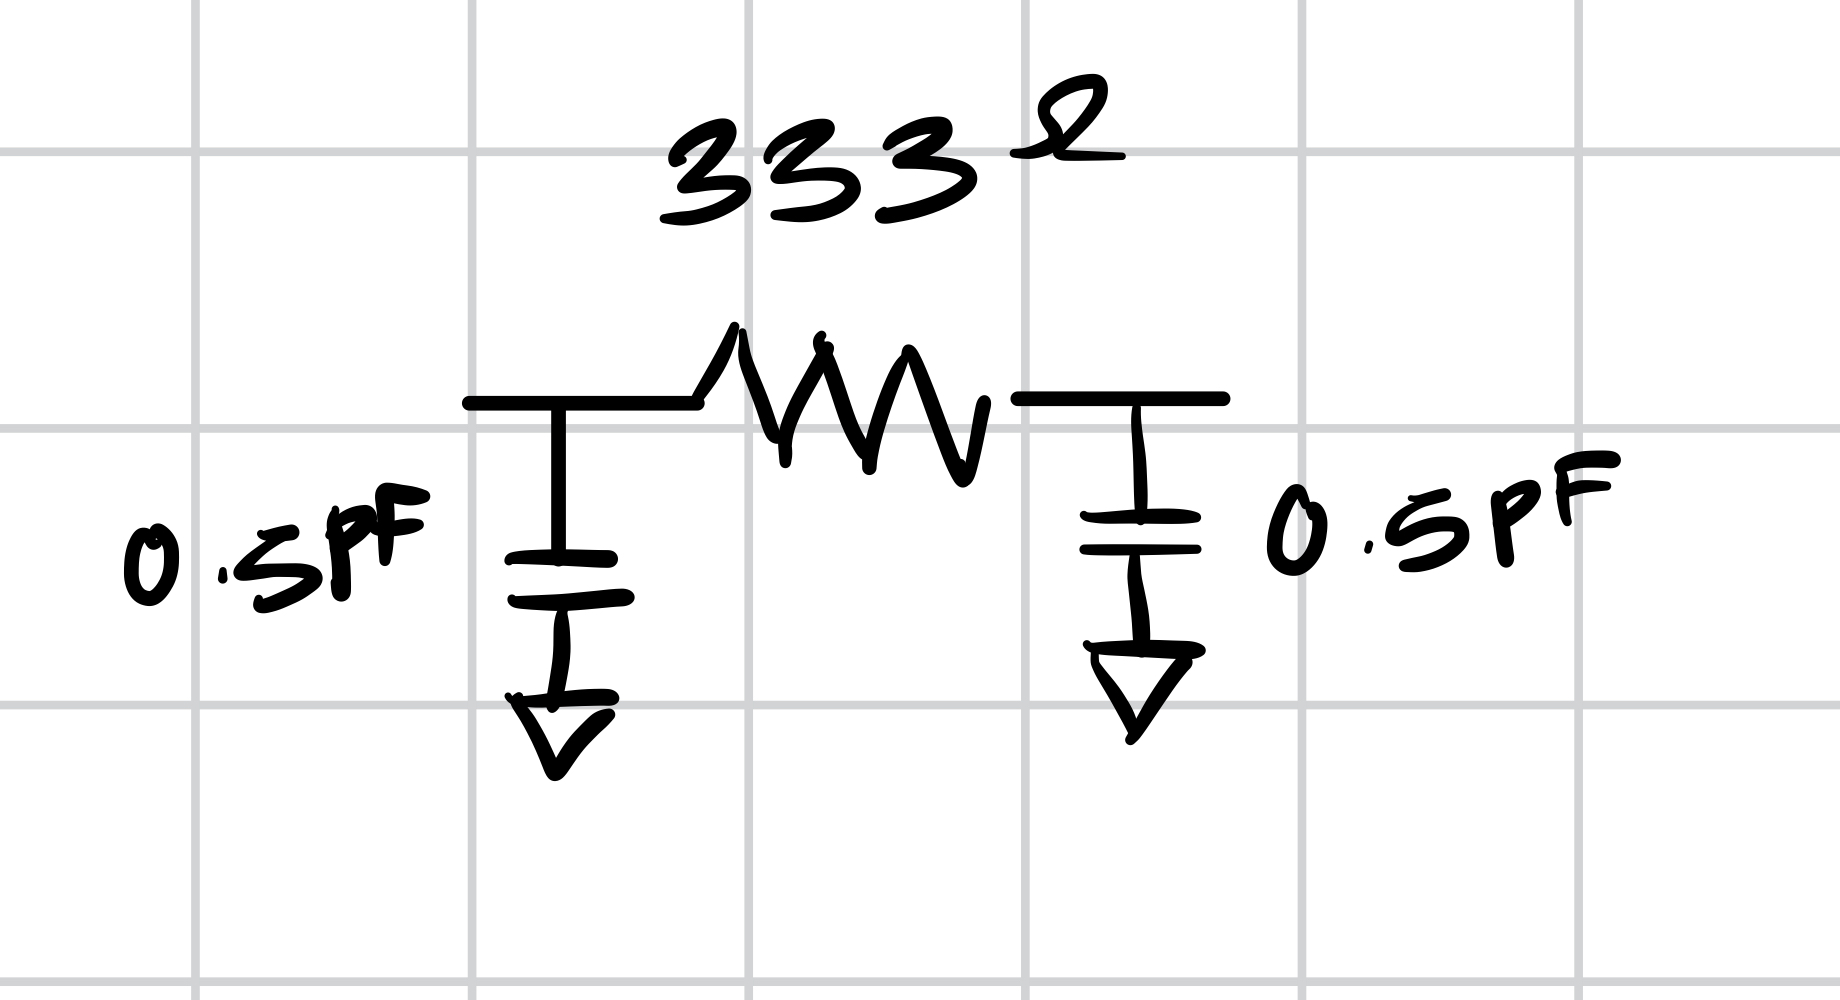
\includegraphics[width=0.4\textwidth]{homework-5_fig-1.jpg}
  \caption{\(\pi\)-model representation}
  \label{fig:pi-model}
\end{figure}
\end{enumerate}
\renewcommand{\thesubsection}{\thesection.\Alph{subsection}}
\begin{enumerate}[label=\thesubsection]
	\setcounter{subsection}{1}
	\item First, we can model the process of crosstalk between a switching and non-switching wire as a capacitive voltage divider by assuming the victim wire is floating (we'll correct for this assumption momentarily). In the above case, 
		\[
			\Delta V_{\mathrm{victim}} = \frac{C_{\mathrm{adj}}}{C_{\mathrm{gnd-v}} + C_{\mathrm{adj}}} \Delta V_{\mathrm{agressor}}. = \frac{0.12}{0.2} = 0.6 \ \mathrm{V}.
		\]
		Therefore, in a floating, non-switching victim wire, we'd expect to see a peak change of \(0.4 \ \mathrm{V}\) in the victim wire for a corresponding \(1 \ \mathrm{V}\) change in the agressor wire. 

		In our case, however, the victim wire is not floating; instead, it is driven by an inverter of equal resistance to the agressor wire. Under these conditions, the victim's driver will supply current to oppose and reduce the undesireable voltage spike, proportional to the time constant ratio \(k\) of the agressor to the victim. Since both victim and agressor in this case have an identical time constant \(\tau\), \(k=1\), and the peak change in the victim wire may be expressed as 
		\[
			\Delta V_{\mathrm{victim}} = 0.4 \times \frac{1}{1+k} = 0.3 \ \mathrm{V}.
		\]
	\setcounter{subsection}{2}
	\item 
		\begin{enumerate}[label=\arabic*.]
			\item Assuming traditional unit inverters with \(p_{\mathrm{inv}} \approx 1\) and assuming \(\tau = RC = 50 \ \mathrm{ps}\), \(R_w = 320 \ \ohm\), and \(C_w = 0.12 \ \mathrm{pF}\) then
					\[
						\frac{t_{pd}}{l} = (4\sqrt{RCR_wC_w}) = 4 \sqrt{(50 \ \mathrm{ps})(320 \ \ohm/\mathrm{mm})(0.12 \ \mathrm{pF/mm})} = 175 \ \mathrm{ps/mm}.
					\]
			\item The best length of wire between repeaters may be found as 
					\[
						\frac{l}{N} = 2\sqrt{\frac{RC}{R_w C_w}} = 2\sqrt{\frac{50 \ \mathrm{ps}}{(320 \ \ohm/\mathrm{mm})(0.12 \ \mathrm{pF/mm})}}=2.28 \ \mathrm{mm}.
					\]
		\end{enumerate}
\end{enumerate}
\end{document} 
